\documentclass{beamer}
%\usepackage[latin1]{inputenc}

\usepackage[utf8]{inputenc}
\usepackage{polski}
\usepackage{graphicx}

\usetheme{Warsaw}
\title[Sieci Bayesowskie]{Uczenie modeli kanonicznych w sieciach Bayesowsich - efektywne uczenie modelu Noisy OR/MAX z danych.}
\author{Krzysztof Nowak}
\institute{Politechnika Białostocka}
\date{23.10.2012}
\begin{document}

\begin{frame}
\titlepage
\end{frame}

\begin{frame}{Wprowadzenie}
	Sieć Bayesowska - struktura służąca do przedstawiania zależności pomiędzy zdarzeniami bazując na rachunku prawdopodobieństwa.


	\pause W sieciach bayesowskich można wyróżnić:
	\begin{itemize}
		\pause \item Strukturę sieci - skierowany, acykliczny graf
		\pause \item Parametry sieci - wartości liczbowe określające prawdopodobieństwo poszczególnych zdarzeń
	\end{itemize}
	
\end{frame}

\begin{frame}{Struktura sieci}
	\begin{figure}[h!]
		\centering
		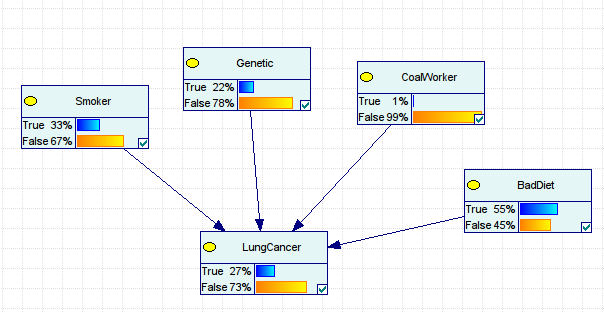
\includegraphics[width=10cm]{1.png}
		\caption{Przykładowa sieć bayesowska - Genie 2.0}
	\end{figure}
\end{frame}

\begin{frame}{Parametry sieci}
	CPT - Conditional Probability Table
	\begin{figure}[h!]
		\centering
		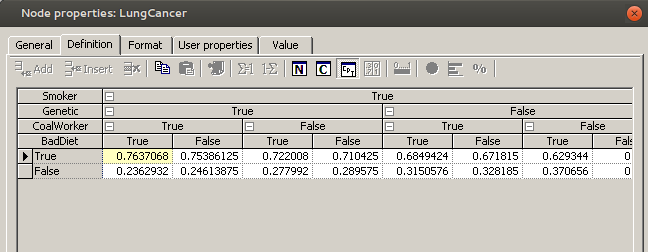
\includegraphics[width=10cm]{2.png}
		\caption{CPT - Genie 2.0}
	\end{figure}
	\begin{itemize}
		\item Wykładniczy przyrost parametrów ze względu na ilość węzłów rodzicielskich.
	\end{itemize}
\end{frame}

\begin{frame}{Parametry sieci}
	\begin{figure}[h!]
		\centering
		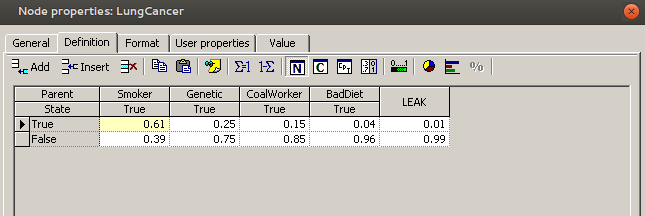
\includegraphics[width=10cm]{3.png}
		\caption{Noisy MAX/OR - Genie 2.0}
	\end{figure}

	\begin{itemize}
		\item Liniowy przyrost parametrów ze względu na ilość węzłów rodzicielskich.
		\item Bramka Noisy OR jest szczególnym przypadkiem bramki Noisy MAX.
	\end{itemize}
\end{frame}

\begin{frame}{Modele kanoniczne - Noisy OR}
	\begin{itemize}
		\item Najprostszy i najbardziej intuicyjny z modeli kanonicznych.
	\end{itemize}
	Bramka Noisy-OR wymaga podania prawdopodobieństwa wystąpienia danego zjawiska dla poszczególnych wartości węzłów rodzicielskich, niezależnie od pozostałych:
	\begin{equation}
		p_k = P(y|\bar{x}_1, \bar{x}_2, ... , x_k, ... , \bar{x}_{n-1}, \bar{x}_n).
	\end{equation}
	Prawdopodobieństwo w bramce Noisy-OR przy wektorze wejściowym $\textbf{X}$ wyliczamy następująco:
	\begin{equation}
		P(y|\textbf{X}) = 1 - \prod_{i:x_i\epsilon \textbf{X}}(1-p_i)
	\end{equation}

	Parametr ``LEAK'' oznacza prawdopodobieństwo wystąpienia danego zjawiska, pomimo braku wystąpienia jakiejkolwiek jawnej przyczyny. 
	Służy on do uwzględnienia tzw. niewymodelowanych przypadków:

	\begin{equation}
		p_{leak} = P(y|\bar{x}_1, \bar{x}_2, ... , \bar{x}_n).
	\end{equation}
\end{frame}

\begin{frame}{Wyliczanie parametrów z danych - CPT}
	Standardowy węzeł w sieci bayesowskiej wymaga podania całej tabeli prawdopodobieńst warunkowych. 
	Zliczamy poszczególne wystąpienia danych kombinacji parametrów w pliku z danymi i na ich podstawie wyliczamy prawdopodobieństwo.

	\begin{figure}[h!]
		\centering
		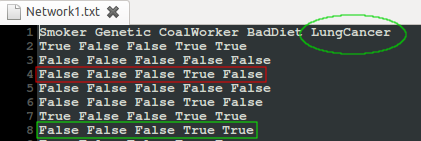
\includegraphics[width=10cm]{4.png}
		\caption{Przykładowy plik z danymi}
	\end{figure}
	\begin{equation}
	\frac{\textcolor{green}{27}}{\textcolor{green}{27} + \textcolor{red}{311}} = 0.079
	\end{equation}
\end{frame}	
\begin{frame}{Wyliczanie parametrów z danych - Noisy-OR/MAX}
	\begin{itemize}
		\item Węzeł typu Noisy-OR/MAX nie wymaga podania prawdopodobieństwa dla każdej możliwej kombinacji parametrów, a jedynie dla prawdopodobieństwa wystąpienia każdego z parametrów z osobna (niezależnie od innych).
		\item Sposób wyliczania jest identyczny, jednak ze względu na charakter bramki Noisy-OR/MAX potrzebujemy znacznie mniej parametrów.
	\end{itemize}
\end{frame}

\begin{frame}{Usprawnienie wyliczania parametrów z danych - Noisy-OR/MAX}
	\begin{itemize}
		\item W podanej wcześniej sieci, ilość rekordów składających się na wyliczenie wszystkich parametrów dla bramki Noisy-OR to około \textbf{47\%}.
		\item Można to interpretować w taki sposób: Przy określaniu parametrów dla bramki Noisy-OR, pomijamy \textbf{53\%} informacji zawartych w pliku z danymi.
		\item Dla porównania, określenie parametrów (CPT) dla bramki standardowej wykorzystuje cały plik z danymi.
		\pause \item Czy da się lepiej uzyskać poszczególne parametry sieci Noisy-OR ?
	\end{itemize}
\end{frame}

\begin{frame}{Usprawnienie wyliczania parametrów z danych.}
	\begin{itemize}
		\item Układy równań parametrów.
		\pause \item Wybieramy układ $n$ niewiadomych TODO<-
	\end{itemize}
\end{frame}

\begin{frame}{Wyniki}
	\begin{figure}[h!]
		\centering
		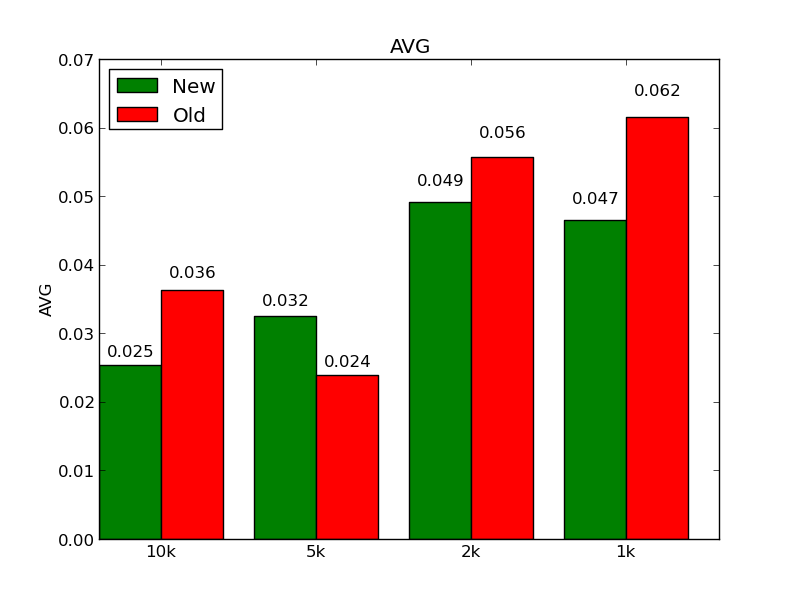
\includegraphics[width=9cm]{avg.png}
		\caption{Średni błąd parametru}
	\end{figure}
\end{frame}

\begin{frame}{Wyniki}
	\begin{figure}[h!]
		\centering
		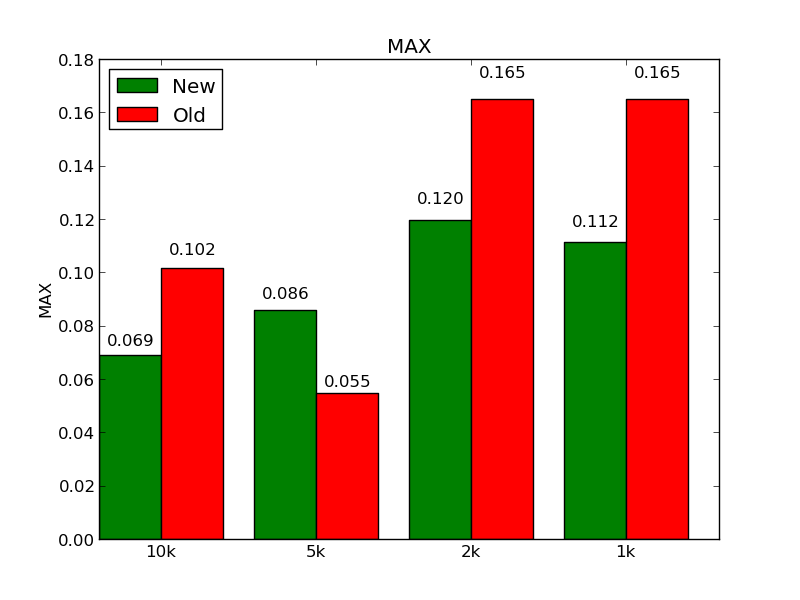
\includegraphics[width=9cm]{max.png}
		\caption{Maksymalny błąd parametru}
	\end{figure}
\end{frame}

\begin{frame}{Wyniki}
	\begin{figure}[h!]
		\centering
		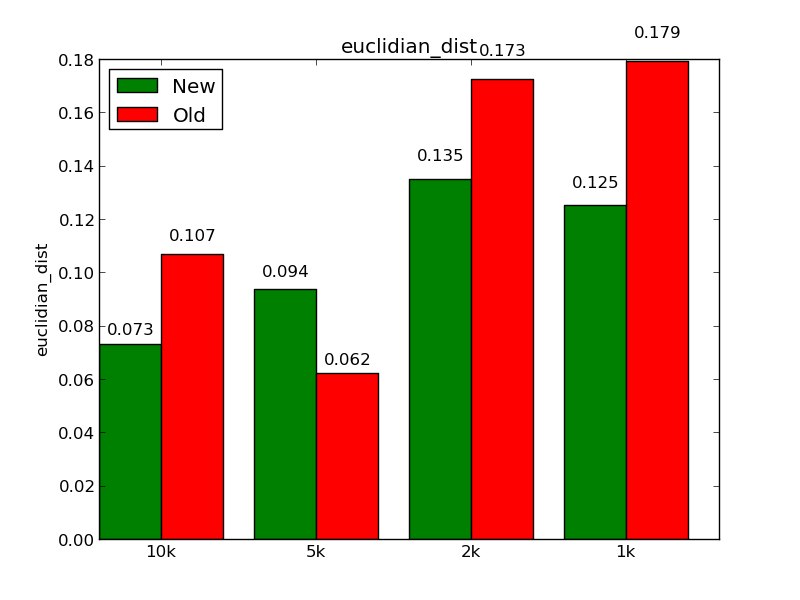
\includegraphics[width=9cm]{euclidian_dist.png}
		\caption{Odległość euklidesowa wektoru prawdopodobieńst przybliżonych od wzorcowych.}
	\end{figure}
\end{frame}

\begin{frame}{Wyniki}
	\begin{figure}[h!]
		\centering
		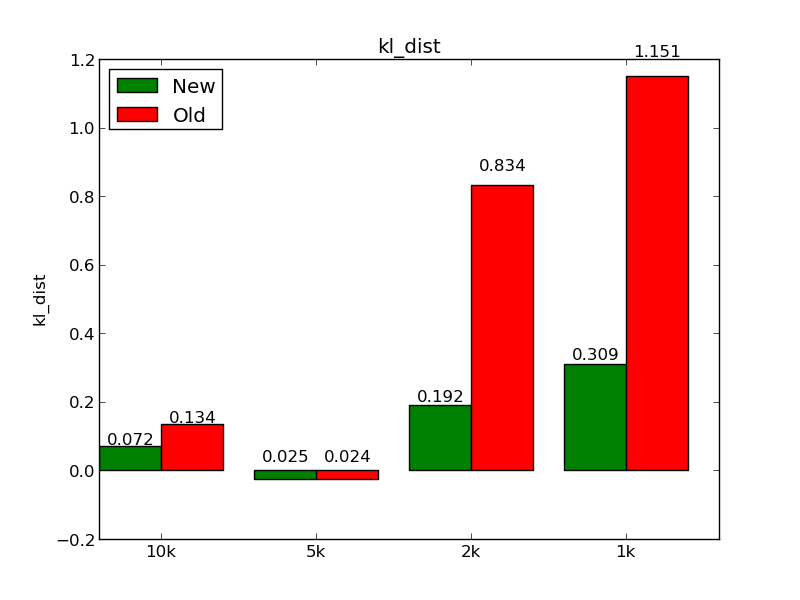
\includegraphics[width=9cm]{kl_dist.png}
		\caption{Dywergencja Kullbacka-Leiblera.}
	\end{figure}
\end{frame}

\begin{frame}{Wyniki}
	\begin{figure}[h!]
		\centering
		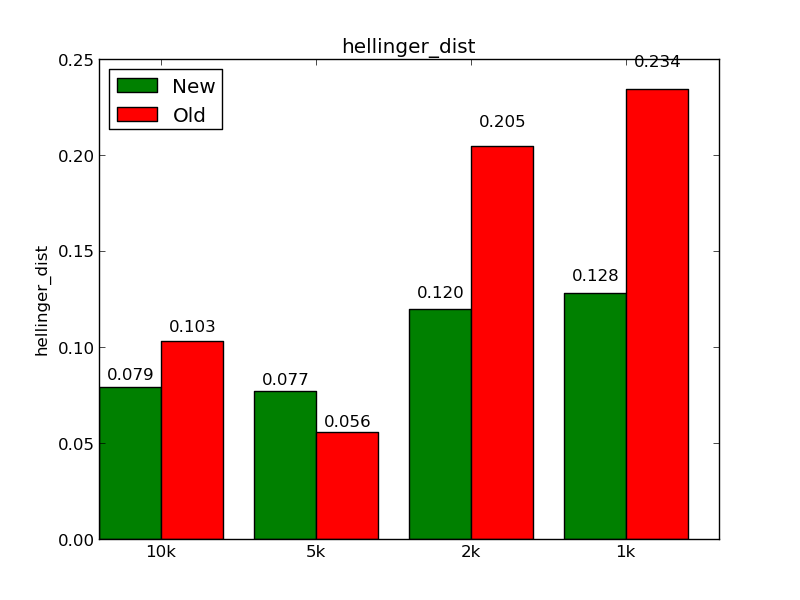
\includegraphics[width=9cm]{hellinger_dist.png}
		\caption{Odległość Hellingera.}
	\end{figure}
\end{frame}



\begin{frame}{Źródła}
	\begin{itemize}
		\item Francisco J. Diez, Marek J. Drużdżel - "Canonical Probabilistic Models for Knowledge Engineering" (28.4.2007)
		\item Nir Friedman, Moises Goldszmidt - "Learning Bayesian networks with local structure"
		\item Agnieszka Oniśko, Marek J. Drużdżel, Hanna Wasyluk - "Learning Bayesian network parameters from small data sets: application of Nosiy-OR gates" (1.3.2001)
	\end{itemize}
\end{frame}
\end{document}
